\chapter{Iteración 8}

\begin{abstract}
Esta iteración se orienta al cierre de la experiencia de partida. Las funcionalidades
previstas siguen siendo victoria, derrota y una segunda revisión visual de
\textit{sprites}, pero en el estado actual de desarrollo la iteración apenas se ha
iniciado y solo incorpora un primer ajuste técnico sobre la progresión entre círculos.
\end{abstract}

\section{Lista de funcionalidades}
La octava iteración se plantea como una fase de cierre sobre la base ya consolidada en las
entregas anteriores. Después de haber reforzado combate, enemigos, progresión por círculos,
inventario y salas especiales, el proyecto necesita resolver qué ocurre cuando la partida se
gana o se pierde, y cómo se presenta ese estado final al jugador. Por ello, esta iteración se
estructura en torno a tres funcionalidades: victoria, derrota y una segunda actualización de
\textit{sprites} orientada a unificar el acabado visual del juego. No obstante, a fecha de
esta documentación la iteración está todavía en arranque y el único avance técnico ya
integrado consiste en restringir la bajada de círculo hasta haber obtenido la llave
correspondiente.

\begin{enumerate}
\item \textbf{Victoria.} Esta funcionalidad recogerá la lógica necesaria para detectar el
cierre exitoso de la partida y trasladar al jugador a un estado final reconocible. Su alcance
incluye decidir cuándo una \textit{run} debe considerarse completada, congelar el flujo de
juego de forma controlada y mostrar una transición clara hacia la pantalla o capa visual de
victoria. En términos funcionales, esta feature cerrará el bucle principal del juego, evitando
que la progresión por círculos termine en un estado ambiguo o sin recompensa explícita.

\begin{figure}[H]
\begin{center}
\missingfigure{Sustituir por captura representativa del flujo de Victoria en la iteración 8}
% \includegraphics[width=.9\textwidth]{figures/iteracion8_victoria.png}
\caption{Resultado visual previsto de la feature Victoria en la iteración 8}
\label{fig:iteracion8-feature-victoria}
\end{center}
\end{figure}

\item \textbf{Derrota.} Esta funcionalidad introducirá el comportamiento asociado a la
derrota del jugador cuando la partida no pueda continuar. Su alcance abarca la detección de
la condición de derrota, la detención o atenuación del bucle jugable y la presentación de un
flujo de reinicio o retorno a menú coherente con el resto de sistemas ya presentes. En la
práctica, esta feature completa la gestión de estados de partida, permitiendo que el fracaso
tenga una respuesta controlada, legible y reutilizable.

\begin{figure}[H]
\begin{center}
\missingfigure{Sustituir por captura representativa del flujo de Derrota en la iteración 8}
% \includegraphics[width=.9\textwidth]{figures/iteracion8_derrota.png}
\caption{Resultado visual previsto de la feature Derrota en la iteración 8}
\label{fig:iteracion8-feature-derrota}
\end{center}
\end{figure}

\item \textbf{Actualizar Sprites (II).} Esta funcionalidad constituye la segunda parte de la
feature \textit{Actualizar Sprites}, cuya primera entrega se realizó en la iteración 5. En
esta ocasión, el alcance ya no se limita al ritmo de animación del jugador, sino que se
orienta a unificar la identidad gráfica de \gls{hud}, menús y pantallas de cierre de partida.
Su objetivo es que los nuevos estados de victoria y derrota no se perciban como capas
aisladas, sino como una extensión natural del lenguaje visual ya usado en \textit{Via
Inferni}. En términos funcionales, esta feature no introduce nueva mecánica, pero sí mejora
la claridad y la cohesión con la que el jugador interpreta el estado de la partida.

\begin{figure}[H]
\begin{center}
\missingfigure{Sustituir por captura representativa de Actualizar Sprites (II) en la iteración 8}
% \includegraphics[width=.9\textwidth]{figures/iteracion8_actualizar_sprites_ii.png}
\caption{Resultado visual previsto de la feature Actualizar Sprites (II) en la iteración 8}
\label{fig:iteracion8-feature-sprites}
\end{center}
\end{figure}
\end{enumerate}

La combinación de estas tres funcionalidades hace que la octava iteración actúe como cierre
de la experiencia jugable. Si en iteraciones anteriores el foco estaba en construir sistemas,
aquí el objetivo pasa a ser cerrar el ciclo completo de la partida y presentarlo con una
identidad visual más consistente.

\section{Diseño}
El diseño de esta iteración parte de una necesidad de cierre. El proyecto ya dispone de una
partida suficientemente completa para explorar, combatir, progresar y descender por círculos,
pero todavía necesita definir con claridad cómo termina esa experiencia y cómo se comunica ese
final al jugador. La idea dominante es resolver esos estados finales sin introducir flujos
paralelos innecesarios y reutilizando, siempre que sea posible, las piezas de interfaz y
control de escena ya existentes. Como paso previo, ya se ha empezado a reforzar la progresión
entre círculos obligando a validar la llave antes del descenso, de modo que el final de cada
tramo de la \textit{run} quede mejor controlado.

\subsection{Diseño de la victoria}
La victoria se diseñará como un estado terminal explícito del flujo de partida. La decisión
principal consiste en no tratarla como una mera transición de escena desconectada del sistema
de progresión, sino como una consecuencia directa del avance del jugador por los círculos y de
la resolución del último objetivo de la \textit{run}.

Por ello, el diseño de esta funcionalidad debe separar dos responsabilidades: por un lado, la
detección de que la partida ha terminado con éxito; por otro, la presentación visual y las
acciones disponibles una vez alcanzado ese estado. Esta separación facilitará que la lógica de
fin de partida pueda mantenerse estable aunque cambie el diseño de la interfaz final.

\subsection{Diseño de la derrota}
La derrota se diseñará con un criterio simétrico al de la victoria, pero atendiendo a que su
activación depende del estado del jugador y no del progreso por círculos. La decisión
importante aquí es evitar una derrota difusa, donde el jugador simplemente deje de controlar
al personaje sin una transición clara.

Por ello, el diseño debe contemplar un flujo que capture la pérdida de la partida, desactive
la interacción jugable principal y exponga salidas claras, como reiniciar la \textit{run} o
volver al menú principal. Esto permite que la derrota actúe como una respuesta del sistema y
no como un fallo silencioso del juego.

\subsection{Diseño de Actualizar Sprites (II)}
La segunda revisión visual se diseña como una capa de cohesión, no como una sustitución
aislada de recursos. La decisión central es que los nuevos estados de victoria y derrota
compartan la misma dirección visual que \gls{hud}, menús y elementos ya consolidados, en
lugar de introducir estilos desconectados entre sí.

Esto implica revisar tanto iconografía y paneles como la legibilidad de retratos, botones y
composiciones visuales asociadas al cierre de partida. El objetivo no es solo mejorar el
aspecto visual, sino hacer que el jugador identifique con mayor claridad en qué estado se
encuentra el juego.

\section{Implementación}
La implementación de esta iteración previsiblemente se apoyará en una capa de coordinación del
estado de partida y en ajustes sobre la interfaz ya existente. Aunque las tres features tienen
un peso distinto, comparten la necesidad de integrarse con el flujo actual de escenas, con la
pausa y con el \gls{hud} sin duplicar lógica.

\subsection{Estado actual de implementación}
Por ahora, el único cambio ya incorporado en esta iteración consiste en reforzar la progresión
entre círculos mediante una restricción sobre las escaleras de descenso. Este trabajo se apoya
principalmente en \texttt{CircleKeyPickup}, \texttt{CircleManager}, \texttt{MapGenerator},
\texttt{Room} y \texttt{Stairs}. \texttt{MapGenerator} reserva una sala válida para la llave
del círculo, \texttt{Room} se encarga de instanciar el pickup cuando corresponde y
\texttt{Stairs} solo activa el descenso cuando \texttt{CircleManager} confirma que la llave
actual ha sido recogida.

Se trata todavía de un avance de infraestructura y no del cierre funcional de victoria,
derrota o revisión visual. Su utilidad principal es preparar una progresión más controlada
para las siguientes tareas de la iteración.

\subsection{Implementación prevista de la victoria}
La resolución técnica de la victoria apunta a reutilizar los sistemas de progresión ya
existentes en torno a \texttt{CircleManager}, \texttt{Stairs} y la escena principal de juego.
Sobre esa base, será necesario incorporar un componente coordinador que detecte el cierre
válido de la \textit{run}, congele la simulación y muestre la interfaz final de victoria.

También será necesario conectar ese flujo con acciones posteriores, como reiniciar o volver al
menú principal. En ese sentido, el comportamiento ya presente en \texttt{MainMenuController} y
\texttt{PauseMenuController} ofrece una base útil para no reimplementar navegación de escenas
desde cero.

\subsection{Implementación prevista de la derrota}
La derrota se apoyará previsiblemente en \texttt{Player}, \texttt{PlayerStats} y en los puntos
del sistema donde ya se procesa el daño recibido por el jugador. A partir de ese momento, la
idea es introducir una notificación centralizada que permita pasar de estado jugable a estado
de derrota sin depender de comprobaciones dispersas por distintos scripts.

Una vez detectada la derrota, la interfaz final deberá tomar el control del flujo. Para ello,
resulta razonable reutilizar parte de la lógica de pausa y control de escena ya existente, de
forma que reinicio, retorno al menú y ocultación del \gls{hud} sigan un patrón común.

\subsection{Implementación prevista de Actualizar Sprites (II)}
La segunda revisión visual se apoyará sobre todo en elementos ya existentes como
\texttt{CircleUI}, \texttt{MainMenuController}, \texttt{PauseMenuController} y los recursos
gráficos vinculados a \texttt{PlayerSpriteAnimator} y al \gls{hud}. El objetivo no es abrir un
nuevo sistema visual, sino adaptar y ampliar el ya presente para cubrir los nuevos estados de
final de partida.

Esto puede implicar ajustar \textit{sprites}, paneles, botones, retratos o composiciones de
interfaz, así como asegurar que esos recursos mantienen una escala y una legibilidad
coherentes con el resto del proyecto.

\section{Estado actual y resultados esperados}
El cierre de esta iteración debería dejar resuelto el bucle completo de la partida. Con ello,
el proyecto pasaría de ofrecer una \textit{run} jugable pero abierta a una experiencia capaz de
cerrarse de forma explícita tanto en éxito como en fracaso. En el momento actual, sin embargo,
solo se ha completado el primer ajuste técnico de progresión asociado a la llave de círculo.

De forma resumida, en este punto de la iteración se ha conseguido:

\begin{itemize}
    \item restringir la bajada al siguiente círculo hasta recoger la llave correspondiente;
    \item dejar preparada la base técnica sobre la que apoyar el cierre de la \textit{run}.
\end{itemize}

Al final de la iteración se espera además haber conseguido:

\begin{itemize}
    \item incorporar un flujo claro de victoria asociado al cierre de la \textit{run};
    \item incorporar un flujo claro de derrota asociado a la pérdida del jugador;
    \item reutilizar de forma coherente la navegación entre escenas, reinicio y retorno a menú;
    \item unificar la presentación visual de \gls{hud}, menús y pantallas de cierre de partida;
    \item dejar el proyecto preparado para una entrega final con estados de juego completos.
\end{itemize}

Desde el punto de vista del desarrollo global, esta iteración es importante porque debe
transformar una base jugable completa en una experiencia cerrada. Por ahora, el alcance real
todavía es pequeño y se limita a ese primer ajuste de progresión, de modo que aún no
corresponde atribuir a la iteración un cierre funcional mayor del que realmente tiene.

\begin{figure}[htbp]
\begin{center}
\missingfigure{Sustituir por el diagrama UML de resultado de la iteración 8}
% 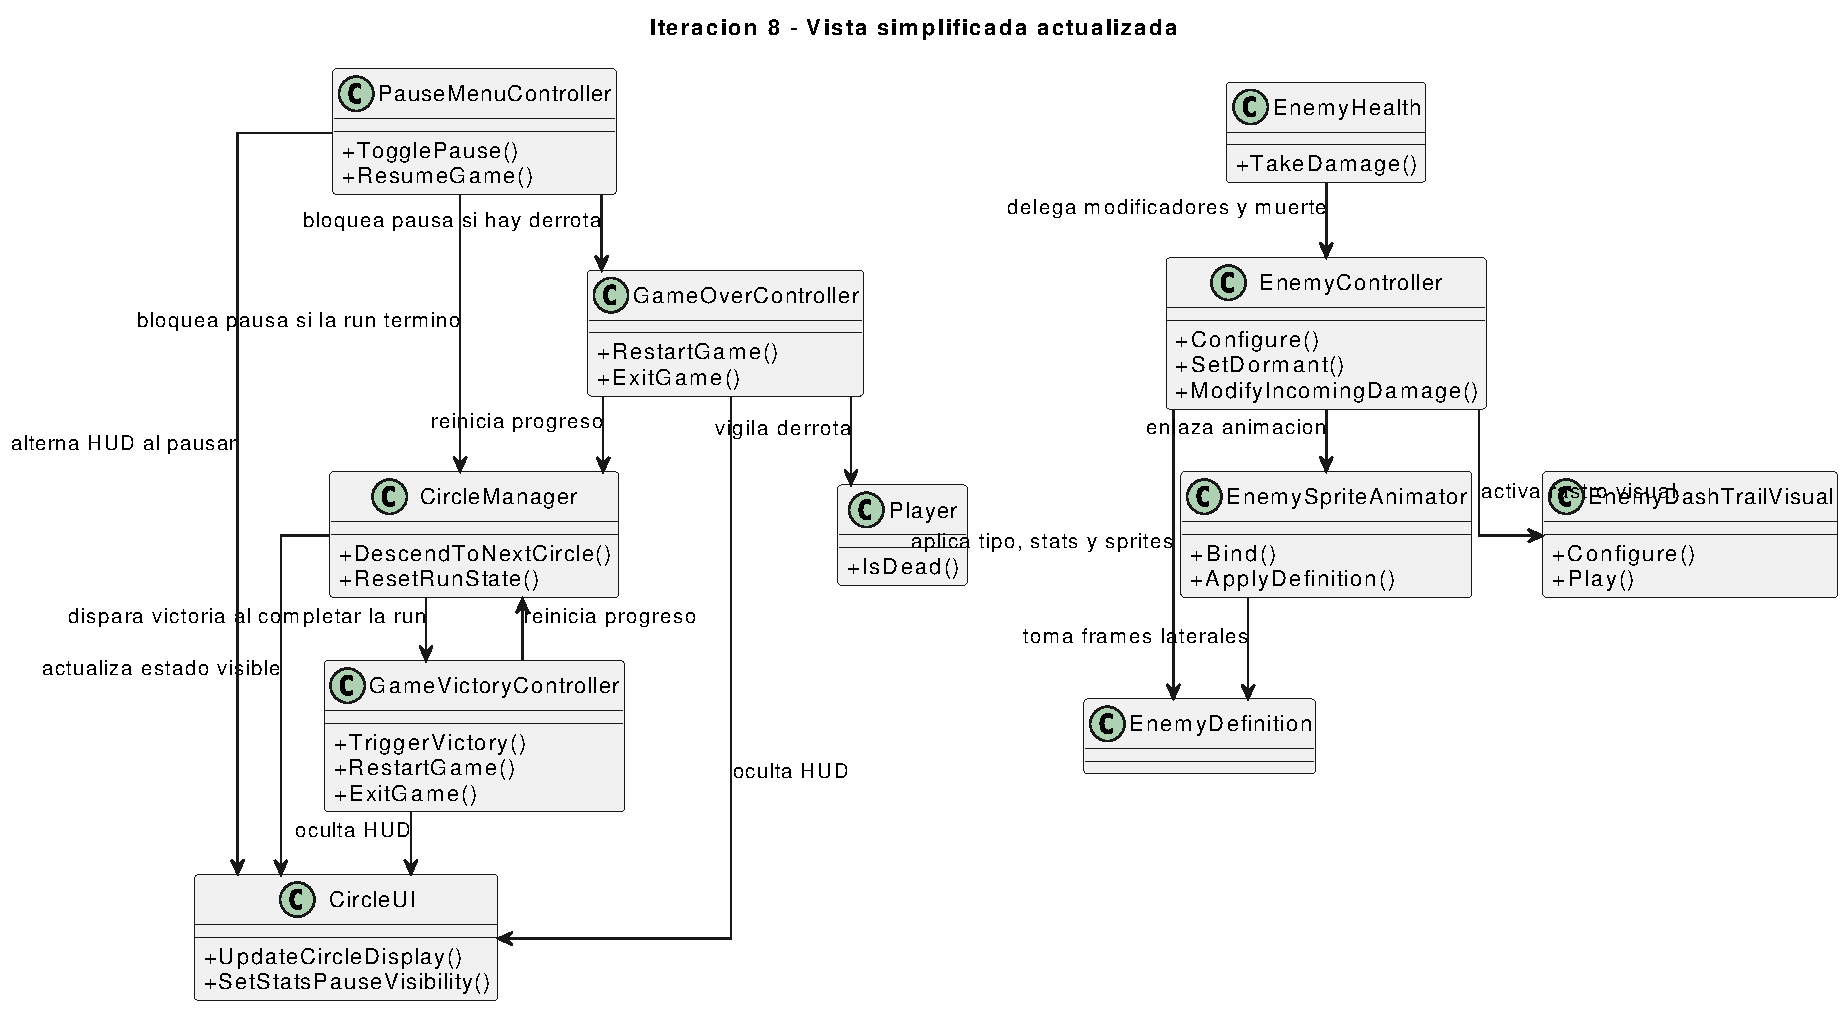
\includegraphics[width=\textwidth]{figures/iteracion8_resultado_uml.pdf}
\caption{Diagrama UML del estado actual de la iteración 8}
\label{fig:uml-resultado-iteracion8}
\end{center}
\end{figure}
